\section{维数论导引}
\label{section:ch08-sec50}

在第 36 节中已经指出过, 若 $X$ 是一个紧致流形, 则对于某一个正整数 $N$, $X$ 可以嵌入到 $\mathbb{R}^{N}$ 中. 本节我们将这一定理推广到任意紧致的可度量化空间.

对任意拓扑空间 $X$, 我们将给出拓扑维数的概念, 这就是最初由 Lebesgue 定义的"覆盖维数". 我们将证明 $\mathbb{R}^{m}$ 的每一个紧致子集的拓扑维数最多是 $m$. 还将证明, 每一个 $m$-维紧致流形的拓扑维数最多是 $m$. (事实上恰好等于 $m$, 不过这一点我们不予证明.)

本节的主要定理是: 任意拓扑维数为 $m$ 的紧致的可度量化空间可以嵌入到 $\mathbb{R}^{N}$ 中, 其中 $N=2m+1$. 这个定理由 K. Menger 和 G. Nöbeling 证得. 这个定理的证明是 Baire 定理的一个应用. 由此得到, 每一个紧致的 $m$-维流形可以嵌入到 $\mathbb{R}^{2m+1}$ 中. 此外, 还可以得到, 对某一个正整数 $N$, 一个紧致的可度量化空间可以嵌入到 $\mathbb{R}^{N}$ 中当且仅当它有有限的拓扑维数.

我们将要做的讨论之中有很大一部分并不要求所涉及的空间是紧致的, 只是为了讨论的方便, 才加上了紧致的限制, 至于这些结果在非紧致情形下的推广, 则放在习题中.

\begin{definition}[集族的阶]
\label{definition:ch08-sec50-order}
空间 $X$ 的一个子集族 $\mathcal{A}$ 称为 $m+1$ \textbf{阶}(order) 的, 如果 $X$ 的某一点属于 $\mathcal{A}$ 的 $m+1$ 个元素之中, 并且 $X$ 的任何点都不会包含在 $\mathcal{A}$ 的多于 $m+1$ 个元素之中.

现在来定义空间 $X$ 的拓扑维数. 前面说过, 对于 $X$ 的一个子集族 $\mathcal{A}$, 子集族 $\mathcal{B}$ 称为\textbf{加细} $\mathcal{A}$ 或 $\mathcal{A}$ 的一个加细, 指的是对 $\mathcal{B}$ 的每一个元素 $B$ 都存在 $\mathcal{A}$ 的一个元素 $A$, 使得 $B\subset A$.

空间 $X$ 称为\textbf{有限维的}(finite dimensional), 如果存在整数 $m$, 使得对于 $X$ 的任意开覆盖 $\mathcal{A}$, 有最多为 $m+1$ 阶的 $X$ 的一个开覆盖 $\mathcal{B}$ 加细 $\mathcal{A}$. $X$ 的\textbf{拓扑维数}(topological dimension) 定义为满足上述要求的 $m$ 的最小值, 记为 $\dim X$.
\end{definition}

\begin{example}
\label{example:ch08-sec50-1}
$\mathbb{R}$ 的任意一个紧致子空间 $X$ 的拓扑维数最多为 $1$. 我们先从定义 $\mathbb{R}$ 的一个 $2$ 阶开覆盖开始. 用 $\mathcal{A}^{1}$ 表示 $\mathbb{R}$ 中所有形如 $(n,n+1)$ 的开区间构成的集族, 其中 $n$ 是整数. 用 $\mathcal{A}^{0}$ 表示 $\mathbb{R}$ 中所有形如 $(n-1/2,n+1/2)$ 的开区间构成的集族, 其中 $n$ 也是整数. 那么 $\mathcal{A}=\mathcal{A}^{0}\cup\mathcal{A}^{1}$ 是 $\mathbb{R}$ 的一个开覆盖, 其中每一个集合的直径为 $1$. 因为在 $\mathcal{A}^{0}$ 和 $\mathcal{A}^{1}$ 中都没有两个元素相交的情况, 所以 $\mathcal{A}$ 是 $2$ 阶的.

现在设 $X$ 为 $\mathbb{R}$ 的任意一个紧致子空间, 给定 $X$ 的一个开覆盖 $\mathcal{C}$, 并且 $\mathcal{C}$ 有一个 Lebesgue 数 $\delta$, 那么 $X$ 的任意直径小于 $\delta$ 的一个子集族都是 $\mathcal{C}$ 的加细. 考虑同胚 $f\colon\mathbb{R}\to\mathbb{R}$, 其中 $f(x)=\left(\frac{1}{2}\delta\right)x$. $\mathcal{A}$ 中的元素在映射 $f$ 下的像构成了 $\mathbb{R}$ 的阶为 $2$ 的开覆盖, 并且这个覆盖中的每一个元素的直径均为 $\frac{1}{2}\delta$, 它们与 $X$ 的交就构成了所要求的 $X$ 的开覆盖.
\end{example}

\begin{example}
\label{example:ch08-sec50-2}
区间 $X=[0,1]$ 的拓扑维数为 $1$. 已知 $\dim X\leqslant 1$, 下面证明等号成立. 设 $\mathcal{A}$ 是由集合 $[0,1)$ 和 $(0,1]$ 构成的 $X$ 的覆盖. 下面证明如果 $\mathcal{B}$ 是 $X$ 的任意一个开覆盖, 加细 $\mathcal{A}$, 那么 $\mathcal{B}$ 至少为 $2$ 阶的. 因为 $\mathcal{B}$ 加细 $\mathcal{A}$, 故它必定包含了不止一个元素. 设 $U$ 是 $\mathcal{B}$ 中的一个元素, $V$ 是其他元素的并. 如果 $\mathcal{B}$ 的阶为 $1$, 那么 $U$ 和 $V$ 是无交的, 由此产生了 $X$ 的一个分割. 因此 $\mathcal{B}$ 的阶数至少为 $2$.
\end{example}

\begin{example}
\label{example:ch08-sec50-3}
$\mathbb{R}^{2}$ 的任意一个紧致子集 $X$ 的拓扑维数最多为 $2$. 为了证明这一点, 我们来构造 $\mathbb{R}^{2}$ 的一个开覆盖 $\mathcal{A}$ 使其阶数为 $3$. 首先, 定义 $\mathcal{A}^{2}$ 是 $\mathbb{R}^{2}$ 中具有以下形式的开的单位正方形构成的集族:
\[
\mathcal{A}^{2}=\{\,(n,n+1)\times(m,m+1)\mid m,n\text{ 是整数}\,\}.
\]
注意 $\mathcal{A}^{2}$ 中的元素是两两无交的. 其次, 取这些正方形之一的每一条 (开) 边 $e$,
\[
e=\{n\}\times(m,m+1)\quad\text{或者}\quad e=(n,n+1)\times\{m\},
\]
并且将其稍加扩大而成为 $\mathbb{R}^{2}$ 中的开集 $U_e$, 使得如果 $e\neq e'$, 那么集合 $U_e$ 和 $U_{e'}$ 无交. 同时还要求所选的每一个 $U_e$ 的直径最多为 $2$. 最后, 定义 $\mathcal{A}^{0}$ 为由所有中心在点 $n\times m$、半径为 $\frac{1}{2}$ 的开球所构成的集族, 如图 \cref{figure:ch08-fig-50-1} 所示.
\end{example}

\par
\begin{figure}[htbp]
\centering
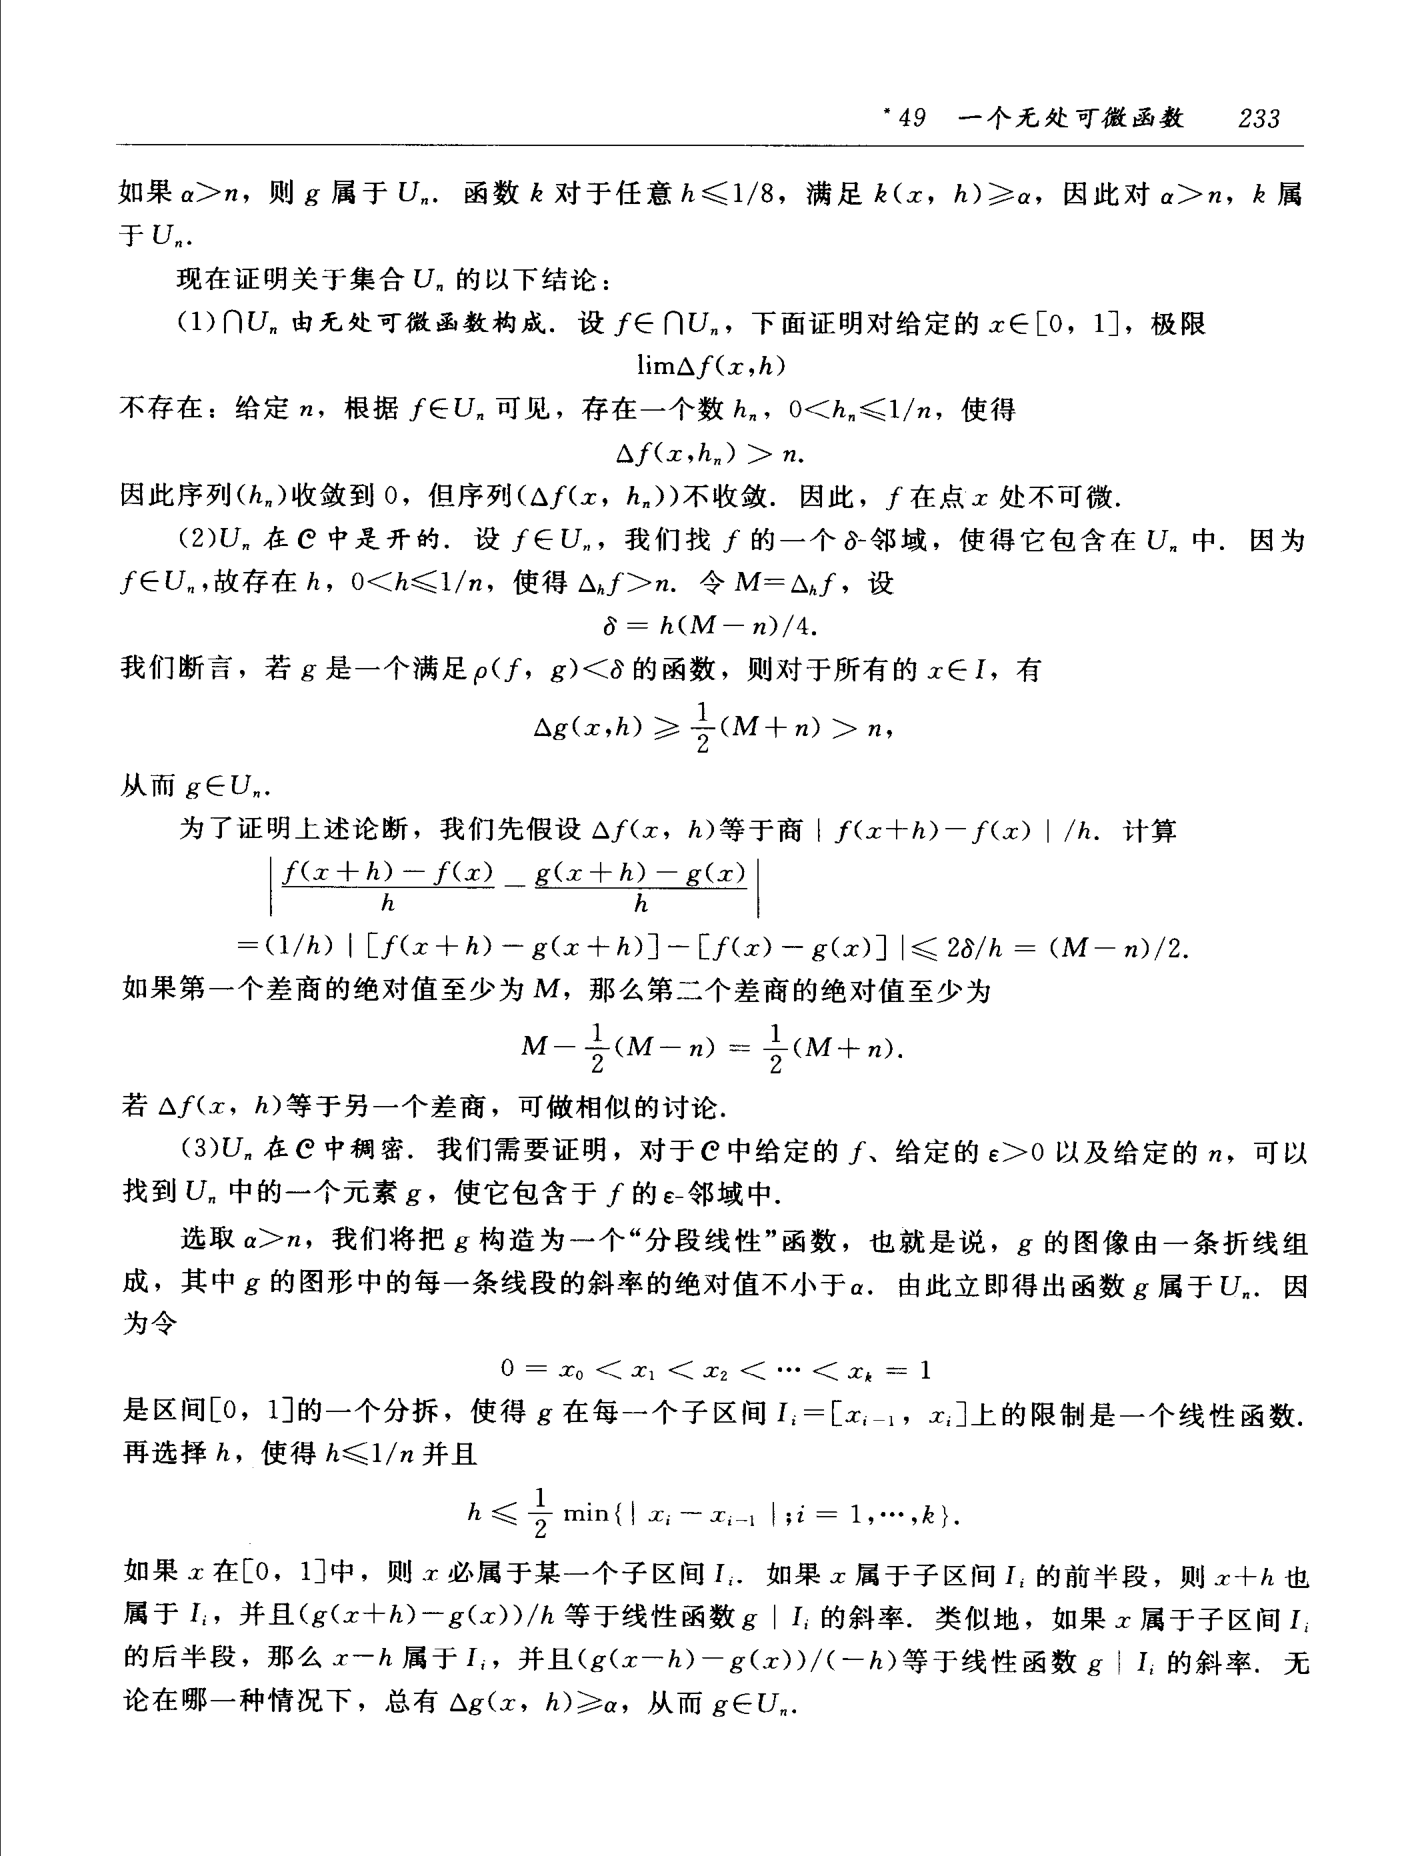
\includegraphics[width=0.8\textwidth]{image/fig-50-1.png}
\caption{$\mathbb{R}^{2}$ 的 $3$ 阶开覆盖.}
\label{figure:ch08-fig-50-1}
\end{figure}

开集族 $\mathcal{A}=\mathcal{A}^{2}\cup\mathcal{A}^{1}\cup\mathcal{A}^{0}$ 覆盖了 $\mathbb{R}^{2}$, 并且它的每一个元素的直径最多为 $2$. 又因为 $\mathbb{R}^{2}$ 中的任何点最多落在每一个 $\mathcal{A}^{i}$ 中的一个集合中, 所以 $\mathcal{A}$ 的阶数为 $3$.

现在设 $X$ 是 $\mathbb{R}^{2}$ 的紧致子空间. 给定 $X$ 的一个开覆盖, 它有一个正的 Lebesgue 数 $\delta$. 考虑同胚 $f\colon\mathbb{R}^{2}\to\mathbb{R}^{2}$, 其中 $f(x)=(\delta/3)x$. 集族 $\mathcal{A}$ 中的开集在 $f$ 之下的像构成了 $\mathbb{R}^{2}$ 的一个开覆盖, 并且其中每一个集合的直径小于 $\delta$. 它们与 $X$ 的交构成了所求的 $X$ 的一个开覆盖.

我们将推广这一结论到 $\mathbb{R}^{n}$ 的紧致子集上.

下列定理给出有关拓扑维数的一些基本结论.

\begin{theorem}
\label{theorem:ch08-sec50-50-1}
设 $X$ 是具有有限维数的一个空间. 如果 $Y$ 是 $X$ 的一个闭子空间, 那么 $Y$ 也具有有限维数, 并且 $\dim Y\leqslant\dim X$.
\end{theorem}

\begin{proof}
设 $\dim X=m$, $\mathcal{A}$ 是由 $Y$ 的开集构成的 $Y$ 的一个覆盖. 对于每一个 $A\in\mathcal{A}$, 选取 $X$ 的一个开集 $A'$, 使得 $A'\cap Y=A$. 这些开集 $A'$ 连同开集 $X-Y$ 一起构成了 $X$ 的一个覆盖. 设 $\mathcal{B}$ 是这个覆盖的一个加细, 同时它也是 $X$ 的一个开覆盖, 并且最多是 $m+1$ 阶的. 于是集族
\[
\{\,B\cap Y\mid B\in\mathcal{B}\,\}
\]
是由 $Y$ 的一个开集构成的 $Y$ 的一个覆盖, 它加细 $\mathcal{A}$ 并且阶数最多为 $m+1$.
\end{proof}

\begin{theorem}
\label{theorem:ch08-sec50-50-2}
设 $X=Y\cup Z$, 其中 $Y$ 和 $Z$ 是 $X$ 中的两个闭子空间, 都具有有限拓扑维数. 那么
\[
\dim X=\max\{\dim Y,\dim Z\}.
\]
\end{theorem}

\begin{proof}
设 $m=\max\{\dim Y,\dim Z\}$. 下面我们证明 $X$ 是有限维的, 并且拓扑维数最多为 $m$. 再根据前述定理便得到 $X$ 的拓扑维数是 $m$ 的结论.

\textbf{第一步}. 如果 $\mathcal{A}$ 是 $X$ 的一个开覆盖, 我们说 $\mathcal{A}$ 在 $Y$ 中的点的阶数最多为 $m+1$, 是指 $Y$ 中的点最多属于 $\mathcal{A}$ 的 $m+1$ 个元素.

下面证明, 如果 $\mathcal{A}$ 是 $X$ 的一个开覆盖, 那么存在 $X$ 的一个开覆盖加细 $\mathcal{A}$, 并且在 $Y$ 中的点的阶数最多为 $m+1$.

为了证明这一点, 考虑集族
\[
\{\,A\cap Y\mid A\in\mathcal{A}\,\}.
\]
它是 $Y$ 的一个开覆盖, 所以它有一个开的加细 $\mathcal{B}$ 覆盖 $Y$, 并且其阶数最多为 $m+1$. 任意给定 $B\in\mathcal{B}$, 选取 $X$ 中的一个开集 $U_B$, 使得 $U_B\cap Y=B$. 选取 $\mathcal{A}$ 中的一个元素 $A_B$, 使得 $B\subset A_B$. 令 $\mathcal{C}$ 是由所有集合 $U_B\cap A_B$ 以及所有集合 $A-Y$ 组成的集族, 其中 $B\in\mathcal{B}$, $A\in\mathcal{A}$, 则 $\mathcal{C}$ 就是所要找的 $X$ 的那个开覆盖.

\textbf{第二步}. 设 $\mathcal{A}$ 是 $X$ 的一个开覆盖. 我们将构造 $X$ 的一个开覆盖 $\mathcal{D}$, 使得 $\mathcal{D}$ 加细 $\mathcal{A}$, 并且它的阶数最多为 $m+1$. 设 $\mathcal{B}$ 为 $X$ 的一个开覆盖, $\mathcal{B}$ 加细 $\mathcal{A}$, 并且在 $Y$ 中的点的阶数最多为 $m+1$. 再设 $\mathcal{C}$ 是 $X$ 的开覆盖, 它加细 $\mathcal{B}$ 并且在 $Z$ 中的点的阶数最多为 $m+1$.

我们用以下方式来构造 $X$ 的一个新的覆盖 $\mathcal{D}$: 定义 $f\colon\mathcal{C}\to\mathcal{B}$ 为对于每一个 $C\in\mathcal{C}$, 取 $f(C)$ 为 $\mathcal{B}$ 中的一个元素, 满足 $C\subset f(C)$. 给定 $B\in\mathcal{B}$, 定义 $D(B)$ 为 $\mathcal{C}$ 中所有满足 $f(C)=B$ 的元素 $C$ 的并. (当然, 如果 $B$ 不在 $f$ 的像中, 则 $D(B)$ 为空集.) 取 $\mathcal{D}$ 为所有集合 $D(B)$ 的族, 其中 $B\in\mathcal{B}$.

现在 $\mathcal{D}$ 加细 $\mathcal{B}$, 这是因为对于每一个 $B$ 有 $D(B)\subset B$. 因此 $\mathcal{D}$ 加细 $\mathcal{A}$. 并且 $\mathcal{D}$ 覆盖 $X$, 这是因为 $\mathcal{C}$ 覆盖 $X$, 并且对于每一个 $C\in\mathcal{C}$ 有 $C\subset D(f(C))$. 下面, 我们证明 $\mathcal{D}$ 最多为 $m+1$ 阶. 假设 $x\in D(B_1)\cap\cdots\cap D(B_k)$, 其中 $D(B_i)$ 是互不相同的. 我们希望能证明 $k\leqslant m+1$. 注意集合 $B_1,\cdots,B_k$ 是互不相同的, 这是因为集合 $D(B_i)$ 互不相同. 又因为 $x\in D(B_i)$, 所以对于每一个 $i$, 可以选取一个集合 $C_i\in\mathcal{C}$, 使得 $x\in C_i$ 并且 $f(C_i)=B_i$. 因为集合 $B_i$ 是互不相同的, 所以集合 $C_i$ 也是互不相同的. 进而, 有
\[
x\in[C_{1}\cap\cdots\cap C_{k}]\subset[D(B_{1})\cap\cdots\cap D(B_{k})]\subset[B_{1}\cap\cdots\cap B_{k}].
\]
如果 $x$ 恰好在 $Y$ 中, 根据 $\mathcal{B}$ 在 $Y$ 的点上最多为 $m+1$ 阶, 可见 $k\leqslant m+1$. 如果 $x$ 恰好在 $Z$ 中, 再根据 $\mathcal{C}$ 在 $Z$ 中的点最多为 $m+1$ 阶, 可见 $k\leqslant m+1$.
\end{proof}

\begin{corollary}
\label{corollary:ch08-sec50-50-3}
设 $X=Y_1\cup\cdots\cup Y_k$, 其中每一个 $Y_i$ 是 $X$ 中的一个闭子空间, 并且是有限维的, 则
\[
\dim X=\max\{\dim Y_{1},\cdots,\dim Y_{k}\}.
\]
\end{corollary}

\begin{example}
\label{example:ch08-sec50-4}
每一个紧致的 $1$-维流形 $X$ 的拓扑维数为 $1$. 空间 $X$ 可以表示成同胚于单位区间 $[0,1]$ 的空间的有限并, 然后应用上述推论便得到了所需的结论.
\end{example}

\begin{example}
\label{example:ch08-sec50-5}
每一个紧致的 $2$-维流形的拓扑维数最多为 $2$. 空间 $X$ 可以表示成同胚于 $\mathbb{R}^{2}$ 中单位闭球的空间的有限并, 再根据前述推论便得到了所需的结论.

一个很自然的问题由此产生: 紧致 $2$-维流形的拓扑维数恰好是 $2$ 吗? 答案是肯定的, 但它的证明却不太容易, 需要以代数拓扑作为工具. 我们将在本书的第二部分证明: $\mathbb{R}^{2}$ 中每一个闭的三角区域的拓扑维数至少为 $2$. (见第 55 节.) 据此可见, $\mathbb{R}^{2}$ 中任何包含一个闭的三角区域的紧致子空间的拓扑维数就为 $2$. 从而, 紧致 $2$-维流形的拓扑维数恰好是 $2$.
\end{example}

\begin{example}
\label{example:ch08-sec50-6}
\textbf{弧}(arc) $A$ 是指同胚于单位闭区间的一个空间. $A$ 的\textbf{端点}(end point) 是指使得 $A-\{p\}$ 和 $A-\{q\}$ 是连通子集的点 $p$ 和 $q$. (有限)\textbf{线性图}(linear graph) $G$ 是指一个 Hausdorff 空间, 它可以表示成有限多段弧的并, 其中每对弧最多交于一个公共端点. 这些弧就称为 $G$ 的\textbf{边}(edge), 这些弧的端点就称为 $G$ 的\textbf{顶点}(vertex). $G$ 的每条边, 因为是紧致的, 所以在 $G$ 中是闭的. 由前述推论可见 $G$ 的拓扑维数是 $1$.

图 \cref{figure:ch08-fig-50-2} 中刻画了两个特殊的线性图. 第一个是通常的"气水电问题"的图示. 第二个被称为"五个顶点的完全图". 它们都不能嵌入到 $\mathbb{R}^{2}$ 中. 尽管这个结论是"显而易见的", 但其证明却不那么容易. 在第 64 节中我们将给出其证明.
\end{example}

\par
\begin{figure}[htbp]
\centering
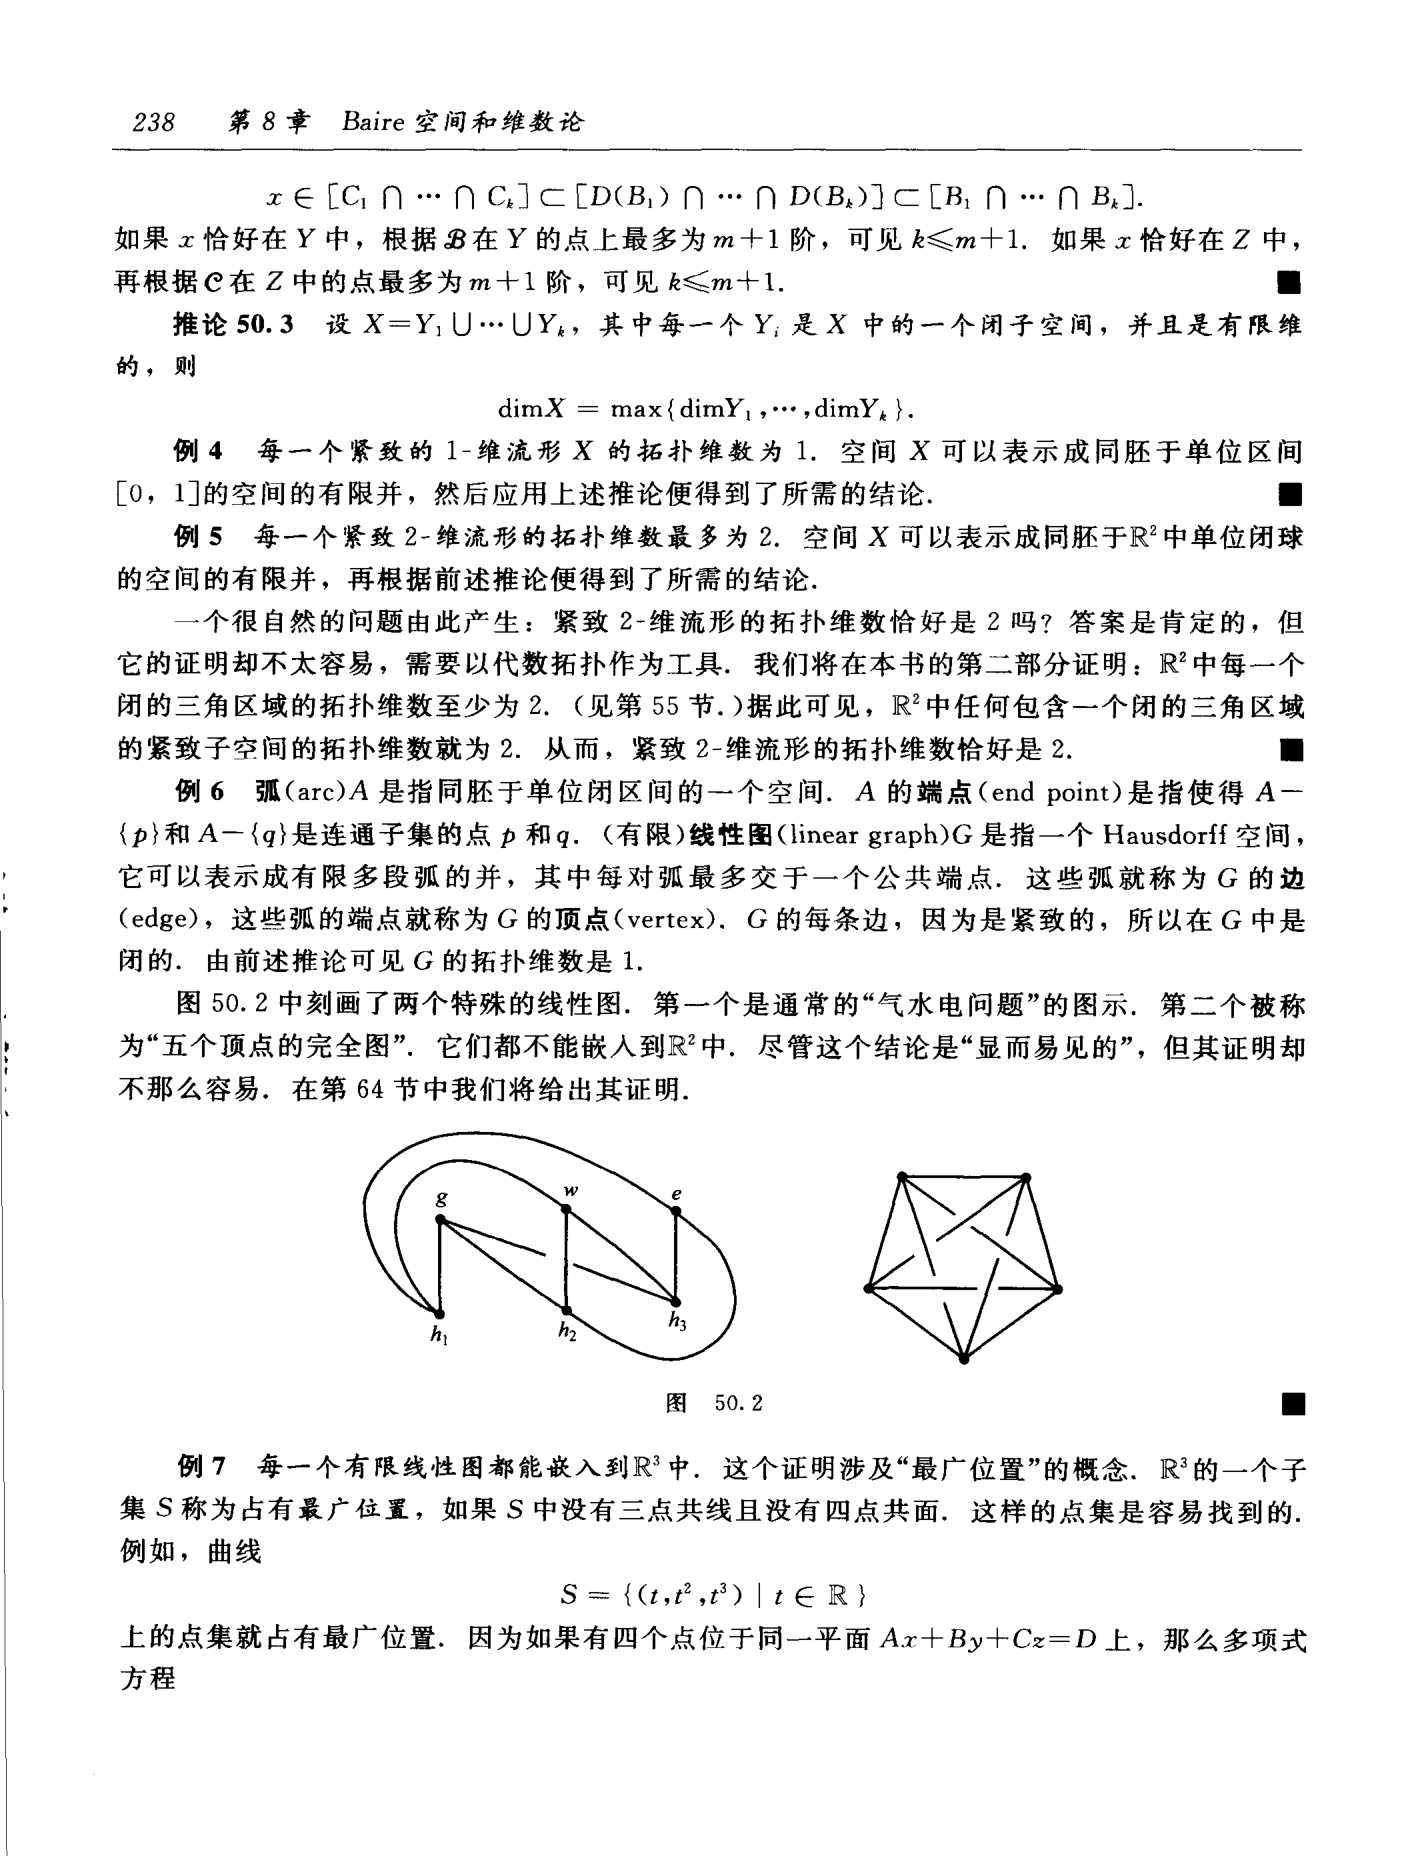
\includegraphics[width=0.7\textwidth]{image/fig-50-2.png}
\caption{两个不能嵌入 $\mathbb{R}^{2}$ 的线性图.}
\label{figure:ch08-fig-50-2}
\end{figure}

\begin{example}
\label{example:ch08-sec50-7}
每一个有限线性图都能嵌入到 $\mathbb{R}^{3}$ 中. 这个证明涉及"最广位置"的概念. $\mathbb{R}^{3}$ 的一个子集 $S$ 称为\textbf{占有最广位置}, 如果 $S$ 中没有三点共线且没有四点共面. 这样的点集是容易找到的. 例如, 曲线
\[
S=\{\,(t,t^{2},t^{3})\mid t\in\mathbb{R}\,\}
\]
上的点集就占有最广位置. 因为如果有四个点位于同一平面 $Ax+By+Cz=D$ 上, 那么多项式方程
\[
At+Bt^{2}+Ct^{3}=D
\]
将有四个不同的实根! 如果有三点共线, 那么可以取 $S$ 中另外一个点, 获得位于同一平面上的四个点.

现在给定一个有限线性图 $G$, 其顶点分别是 $v_1,\cdots,v_n$, 选取 $\mathbb{R}^{3}$ 中占有最广位置的一个点集 $\{z_1,\cdots,z_n\}$. 定义映射 $f\colon G\to\mathbb{R}^{3}$, 使得 $f$ 将顶点 $v_i$ 映为 $z_i$, 并将连接 $v_i$ 和 $v_j$ 的边同胚地映射到直线的连接 $z_i$ 和 $z_j$ 的那条线段上. 现在 $G$ 的每条边在 $G$ 中都是闭的, 从而根据黏结引理可见, $f$ 是连续的. 下面我们证明 $f$ 是一个单射, 从而说明 $f$ 是一个嵌入. 设 $e=v_iv_j$ 和 $e'=v_kv_m$ 是 $G$ 的两条边. 如果它们没有公共的顶点, 那么 $f(e)$ 和 $f(e')$ 无交. 因为如果有交, 那么 $z_i,z_j,z_k,z_m$ 共面. 如果 $e$ 和 $e'$ 有公共的顶点, 不妨设 $i=k$, 那么 $f(e)$ 和 $f(e')$ 只能交于一点 $z_i=z_k$, 因为如若不然, 就有 $z_i,z_j,z_m$ 共线.
\end{example}

现在, 我们证明一个更一般的嵌入定理: 每一个拓扑维数是 $m$ 的紧致可度量化空间都可以嵌入到 $\mathbb{R}^{2m+1}$ 中. 这个定理又是一个"深刻"的定理. 它并非显而易见的, 例如, 为什么取 $2m+1$ 为这个关键的维数. 这将在证明的过程中进行说明.

为了证明嵌入定理, 我们需要将最广位置的概念推广到 $\mathbb{R}^{N}$ 中. 这将会涉及 $\mathbb{R}^{N}$ 上一些解析几何的知识, 与通常的 $\mathbb{R}^{N}$ 上的线性代数差不多, 只是所用的语言不同而已.

\begin{definition}[几何独立]
\label{definition:ch08-sec50-geom-indep}
$\mathbb{R}^{N}$ 中的一个点集 $\{\boldsymbol{x}_{0},\cdots,\boldsymbol{x}_{k}\}$ 称为\textbf{几何独立的}(geometrically independent) 或\textbf{仿射独立的}(affinely independent), 如果等式
\[
\sum_{i=0}^{k}a_{i}\boldsymbol{x}_{i}=\boldsymbol{0}\quad\text{和}\quad\sum_{i=0}^{k}a_{i}=0
\]
仅在每一个 $a_i=0$ 时才成立.
\end{definition}

显然, 任意单点集是几何独立的. 那么, 一般情况下几何独立意味着什么呢? 如果由第二个等式解出 $a_0$, 再代入第一个等式, 可见这个定义实际上等价于等式
\[
\sum_{i=1}^{k}a_{i}(\boldsymbol{x}_{i}-\boldsymbol{x}_{0})=\boldsymbol{0}
\]
仅在每一个 $a_i=0$ 时才成立. 这恰好是向量空间 $\mathbb{R}^{N}$ 中向量集 $\boldsymbol{x}_1-\boldsymbol{x}_0,\cdots,\boldsymbol{x}_k-\boldsymbol{x}_0$ 线性独立的定义. 这样, 我们就得出了一些直观印象: 任意两个不同的点构成几何独立点集, 不共线的三点构成一个几何独立点集, 在 $\mathbb{R}^{3}$ 中不共面的四点构成几何独立点集, 等等.

由这些说明可见, 下述点
\[
\boldsymbol{0}=(0,0,\cdots,0),\quad
\boldsymbol{\varepsilon}_{1}=(1,0,\cdots,0),\quad\cdots,\quad
\boldsymbol{\varepsilon}_{N}=(0,0,\cdots,1)
\]
在 $\mathbb{R}^{N}$ 中是几何独立的. 另外, $\mathbb{R}^{N}$ 中不存在包含多于 $N+1$ 个点的几何独立点集.

\begin{definition}[由点确定的平面]
\label{definition:ch08-sec50-plane}
设 $\{\boldsymbol{x}_0,\cdots,\boldsymbol{x}_k\}$ 为 $\mathbb{R}^{N}$ 中的一个几何独立点集, 由这些点\textbf{确定的平面} $P$(plane $P$ determined by these points) 定义为 $\mathbb{R}^{N}$ 中所有满足以下条件的点 $\boldsymbol{x}$ 构成的集合:
\[
\boldsymbol{x}=\sum_{i=0}^{k}t_{i}\boldsymbol{x}_{i},\quad\text{其中}\quad\sum_{i=0}^{k}t_{i}=1.
\]
\end{definition}

仅由代数知识即可验证 $P$ 也可以表示为所有点 $\boldsymbol{x}$ 的集合, 其中 $\boldsymbol{x}$ 满足对某一组纯量 $a_1,\cdots,a_k$, 有
\[
\boldsymbol{x}=\boldsymbol{x}_{0}+\sum_{i=1}^{k}a_{i}(\boldsymbol{x}_{i}-\boldsymbol{x}_{0}). \tag{$*$}
\]
这样, $P$ 不仅可以描述成"由点 $\boldsymbol{x}_0,\cdots,\boldsymbol{x}_k$ 确定的平面", 还可以描述成"过点 $\boldsymbol{x}_0$, 并且与向量 $\boldsymbol{x}_1-\boldsymbol{x}_0,\cdots,\boldsymbol{x}_k-\boldsymbol{x}_0$ 平行的平面".

现在考虑定义为 $T(\boldsymbol{x})=\boldsymbol{x}-\boldsymbol{x}_0$ 的同胚 $T\colon\mathbb{R}^{N}\to\mathbb{R}^{N}$, 它称为 $\mathbb{R}^{N}$ 中的一个\textbf{平移}(translation), $(*)$ 式表明映射 $T$ 把平面 $P$ 映到 $\mathbb{R}^{N}$ 的一个向量子空间 $V^k$ 上, 其中 $V^k$ 以向量 $\boldsymbol{x}_1-\boldsymbol{x}_0,\cdots,\boldsymbol{x}_k-\boldsymbol{x}_0$ 为基. 由于这个原因, 常常称 $P$ 为 $\mathbb{R}^{N}$ 中的一个 $k$-\textbf{维平面}($k$-plane).

于是立即可见以下两点: 首先, 如果 $k<N$, $k$-维平面必然在 $\mathbb{R}^{N}$ 中有空内部 (因为 $V^k$ 有空内部). 其次, 如果 $\boldsymbol{y}$ 是 $\mathbb{R}^{N}$ 中不在 $P$ 中的任意一点, 则集合
\[
\{\boldsymbol{x}_{0},\cdots,\boldsymbol{x}_{k},\boldsymbol{y}\}
\]
是几何独立的. 因为若 $\boldsymbol{y}\notin P$, 则 $T(\boldsymbol{y})=\boldsymbol{y}-\boldsymbol{x}_0$ 不在 $V^k$ 中. 根据线性代数中的一个标准定理, 向量 $\{\boldsymbol{x}_1-\boldsymbol{x}_0,\cdots,\boldsymbol{x}_k-\boldsymbol{x}_0,\boldsymbol{y}-\boldsymbol{x}_0\}$ 线性无关, 从而得出我们所期望的结果.

\begin{definition}[占有最广位置]
\label{definition:ch08-sec50-general-pos}
$\mathbb{R}^{N}$ 中的一个点集 $A$ 称为\textbf{在 $\mathbb{R}^{N}$ 中占有最广位置}(general position in $\mathbb{R}^{N}$), 如果 $A$ 的每一个含有 $N+1$ 个点或者少于 $N+1$ 个点的子集都是几何独立的.
\end{definition}

在 $\mathbb{R}^{3}$ 的情形下, 可以验证这与以前的定义是一致的.

\begin{lemma}
\label{lemma:ch08-sec50-50-4}
给定 $\mathbb{R}^{N}$ 的一个有限点集 $\{\boldsymbol{x}_1,\cdots,\boldsymbol{x}_n\}$ 和 $\delta>0$, 存在 $\mathbb{R}^{N}$ 中占有最广位置的一个点集 $\{\boldsymbol{y}_1,\cdots,\boldsymbol{y}_n\}$, 使得对于所有的 $i$, 有 $|\boldsymbol{x}_i-\boldsymbol{y}_i|<\delta$.
\end{lemma}

\begin{proof}
我们采用归纳法证明. 令 $\boldsymbol{y}_1=\boldsymbol{x}_1$, 假定已经给定了 $\mathbb{R}^{N}$ 中占有最广位置的 $\boldsymbol{y}_1,\cdots,\boldsymbol{y}_p$. 考虑 $\{\boldsymbol{y}_1,\cdots,\boldsymbol{y}_p\}$ 中不多于 $N$ 个点的子集确定的 $\mathbb{R}^{N}$ 中的所有平面的集合. 当 $k\leqslant N-1$ 时, 每一个这样的子集都是几何独立的, 并且确定了一个 $k$-维平面. 这些平面在 $\mathbb{R}^{N}$ 中都有空内部. 由于这些平面只有有限多个, 所以它们的并在 $\mathbb{R}^{N}$ 中也有空内部. (注意 $\mathbb{R}^{N}$ 是一个 Baire 空间.) 选取 $\boldsymbol{y}_{p+1}$ 为 $\mathbb{R}^{N}$ 中的一点, 它与 $\boldsymbol{x}_{p+1}$ 的距离不超过 $\delta$, 并且不在上述任何一个平面之中. 由此立即可见集合
\[
C=\{\boldsymbol{y}_{1},\cdots,\boldsymbol{y}_{p},\boldsymbol{y}_{p+1}\}
\]
是 $\mathbb{R}^{N}$ 中占有最广位置的集合. 因为若令 $D$ 为包含 $C$ 中不多于 $N+1$ 个点的一个子集, 当 $D$ 不包含 $\boldsymbol{y}_{p+1}$ 时, 根据归纳假设, $D$ 是几何独立的. 如果 $D$ 含有 $\boldsymbol{y}_{p+1}$, 则 $D-\{\boldsymbol{y}_{p+1}\}$ 包含不多于 $N$ 个点, 并且根据选择, $\boldsymbol{y}_{p+1}$ 不在由这些点所确定的平面中. 于是根据前面所述, $D$ 是几何独立的.
\end{proof}

\begin{theorem}[嵌入定理]
\label{theorem:ch08-sec50-50-5}
每一个拓扑维数为 $m$ 的紧致可度量化空间 $X$ 都可以嵌入到 $\mathbb{R}^{2m+1}$ 中.
\end{theorem}

\begin{proof}
设 $N=2m+1$. 我们用
\[
|\boldsymbol{x}-\boldsymbol{y}|=\max\{\,|x_{i}-y_{i}|\,;\ i=1,\cdots,N\,\}
\]
表示 $\mathbb{R}^{N}$ 上的平方度量. 用 $\rho$ 表示空间 $\mathcal{C}(X,\mathbb{R}^{N})$ 上相应的上确界度量, 其中
\[
\rho(f,g)=\sup\{\,|f(x)-g(x)|\,;\ x\in X\,\}.
\]
因为 $\mathbb{R}^{N}$ 在平方度量下是完备的, 所以在度量 $\rho$ 下, 空间 $\mathcal{C}(X,\mathbb{R}^{N})$ 也是完备的.

选取空间 $X$ 的一个度量 $d$, 因为 $X$ 紧致, 所以 $d$ 是有界的. 给定一个连续映射 $f\colon X\to\mathbb{R}^{N}$, 定义
\[
\Delta(f)=\sup\{\,\operatorname{diam}f^{-1}(\{z\})\mid z\in f(X)\,\}.
\]
数 $\Delta(f)$ 可以测量 $f$ "偏离"单射的程度, 如果 $\Delta(f)=0$, 则每一个集合 $f^{-1}(\{z\})$ 恰好由一个点组成, 因而 $f$ 是一个单射.

现在, 给定 $\varepsilon>0$, 定义 $U_\varepsilon$ 为所有使得 $\Delta(f)<\varepsilon$ 的连续映射 $f\colon X\to\mathbb{R}^{N}$ 的集合, 它是由"偏离"单射的程度小于 $\varepsilon$ 的那些映射组成的. 下面证明 $U_\varepsilon$ 是 $\mathcal{C}(X,\mathbb{R}^{N})$ 中的一个稠密开集. 据此, 交
\[
\bigcap_{n\in\mathbb{Z}_{+}}U_{1/n}
\]
在 $\mathcal{C}(X,\mathbb{R}^{N})$ 中是稠密的, 特别地, 它是非空的.

如果 $f$ 是这个交的一个元素, 那么对任意的 $n$, 有 $\Delta(f)<1/n$. 因此 $\Delta(f)=0$, 从而 $f$ 是单射. 又因为 $X$ 紧致, 所以 $f$ 是一个嵌入. 于是嵌入定理得证.

(1) $U_\varepsilon$ 是 $\mathcal{C}(X,\mathbb{R}^{N})$ 中的一个开集. 给定 $U_\varepsilon$ 中的一个元素 $f$, 我们希望找到以 $f$ 为中心的一个球 $B_\rho(f,\delta)$ 包含于 $U_\varepsilon$. 首先选一个数 $b$, 使得 $\Delta(f)<b<\varepsilon$. 注意, 如果 $f(x)=f(y)=z$, 则有 $x$ 和 $y$ 都属于 $f^{-1}(\{z\})$, 所以 $d(x,y)$ 必小于 $b$. 由此可见, 若令 $A$ 为 $X\times X$ 的子集
\[
A=\{\,x\times y\mid d(x,y)\geqslant b\,\},
\]
则函数 $|f(x)-f(y)|$ 在 $A$ 上是正的. 由于 $A$ 在 $X\times X$ 中是闭的, 所以是紧致的. 于是函数 $|f(x)-f(y)|$ 在 $A$ 上有一个正的极小值. 令
\[
\delta=\frac{1}{2}\min\{\,|f(x)-f(y)|\,;\ x\times y\in A\,\}.
\]
我们断言, 这个 $\delta$ 便足够了.

假设 $g$ 是一个映射, 使得 $\rho(f,g)<\delta$. 如果 $x\times y\in A$, 则根据定义 $|f(x)-f(y)|\geqslant 2\delta$. 这是因为 $g(x)$ 与 $g(y)$ 分别与 $f(x)$ 和 $f(y)$ 的距离小于 $\delta$, 所以必有 $|g(x)-g(y)|>0$. 因此函数 $|g(x)-g(y)|$ 在 $A$ 上是正的. 由此推出, 若 $x$ 和 $y$ 是满足 $g(x)=g(y)$ 的两个点, 则必有 $d(x,y)<b$. 所以 $\Delta(g)\leqslant b<\varepsilon$.

(2) $U_\varepsilon$ 在 $\mathcal{C}(X,\mathbb{R}^{N})$ 中稠密. 这是证明中的困难之处, 需要用到上面讨论过的 $\mathbb{R}^{N}$ 的解析几何知识. 设 $f\in\mathcal{C}(X,\mathbb{R}^{N})$. 给定 $\varepsilon>0$ 和 $\delta>0$, 我们希望找到一个函数 $g\in\mathcal{C}(X,\mathbb{R}^{N})$ 使得 $g\in U_\varepsilon$, 并且 $\rho(f,g)<\delta$.

用有限多个开集 $\{U_1,\cdots,U_n\}$ 覆盖 $X$, 使得
\begin{enumerate}
\item 在 $X$ 中, $\operatorname{diam}U_i<\varepsilon/2$.
\item 在 $\mathbb{R}^{N}$ 中, $\operatorname{diam}f(U_i)<\delta/2$.
\item $\{U_1,\cdots,U_n\}$ 的阶数 $\leqslant m+1$.
\end{enumerate}
设 $\{\phi_i\}$ 是由 $\{U_i\}$ 控制的一个单位分拆 (见第 36 节). 对于每一个 $i$, 选取一个点 $x_i\in U_i$. 再对于每一个 $i$, 选取一个点 $z_i\in\mathbb{R}^{N}$, 使得 $z_i$ 与点 $f(x_i)$ 的距离小于 $\delta/2$, 并且使得 $\{z_1,\cdots,z_n\}$ 在 $\mathbb{R}^{N}$ 中占有最广位置. 最后, 定义 $g\colon X\to\mathbb{R}^{N}$ 为
\[
g(x)=\sum_{i=1}^{n}\phi_{i}(x)\boldsymbol{z}_{i}.
\]
我们断言, $g$ 便是所求的函数.

首先, 我们证明 $\rho(f,g)<\delta$. 注意,
\[
g(x)-f(x)=\sum_{i=1}^{n}\phi_{i}(x)\boldsymbol{z}_{i}-\sum_{i=1}^{n}\phi_{i}(x)f(x).
\]
其中用到了 $\sum\phi_i(x)=1$. 于是
\[
g(x)-f(x)=\sum\phi_{i}(x)(\boldsymbol{z}_{i}-f(x_{i}))+\sum\phi_{i}(x)(f(x_{i})-f(x)).
\]
根据点 $\boldsymbol{z}_i$ 的选取, 对于每一个 $i$, $|\boldsymbol{z}_i-f(x_i)|<\delta/2$. 如果 $i$ 是使得 $\phi_i(x)\neq 0$ 的一个指标, 则有 $x\in U_i$. 因为 $\operatorname{diam}f(U_i)<\delta/2$, 所以 $|f(x_i)-f(x)|<\delta/2$. 由于 $\sum\phi_i(x)=1$, 可见 $|g(x)-f(x)|<\delta$. 于是 $\rho(g,f)<\delta$.

其次, 证明 $g\in U_\varepsilon$. 我们要证明, 若 $x,y\in X$, 并且 $g(x)=g(y)$, 则 $x$ 和 $y$ 同时属于某一个开集 $U_i$, 因而必有 $d(x,y)<\varepsilon/2$. (因为 $\operatorname{diam}U_i<\varepsilon/2$.) 于是 $\Delta(g)\leqslant\varepsilon/2<\varepsilon$.

为此假定 $g(x)=g(y)$, 于是
\[
\sum_{i=1}^{n}[\phi_{i}(x)-\phi_{i}(y)]\boldsymbol{z}_{i}=\boldsymbol{0}.
\]
因为覆盖 $\{U_i\}$ 最多为 $m+1$ 阶, 所以最多有 $m+1$ 个 $\phi_i(x)$ 不为零, 也最多有 $m+1$ 个 $\phi_i(y)$ 不为零. 从而, 和式 $\sum_{i=1}^{n}[\phi_i(x)-\phi_i(y)]\boldsymbol{z}_i$ 最多有 $2m+2$ 个非零项. 注意到和式的系数之和蜕化, 因为
\[
\sum[\phi_{i}(x)-\phi_{i}(y)]=1-1=0.
\]
这些点 $\boldsymbol{z}_i$ 在 $\mathbb{R}^{N}$ 中占有最广位置, 所以其含有不多于 $N+1$ 个元素的任何一个子集必定是几何独立的. 根据假设 $N+1=2m+2$. 于是对于所有的 $i$,
\[
\phi_{i}(x)-\phi_{i}(y)=0.
\]
对某一个 $i$, $\phi_i(x)>0$, 所以 $x\in U_i$. 因为 $\phi_i(y)=\phi_i(x)$, 所以也有 $y\in U_i$.
\end{proof}

为了充实嵌入定理的内涵, 我们需要一些有限维空间的例子. 为此, 我们证明以下定理.

\begin{theorem}
\label{theorem:ch08-sec50-50-6}
$\mathbb{R}^{N}$ 的每一个紧致子空间的拓扑维数最多为 $N$.
\end{theorem}

\begin{proof}
这个证明是例 3 中对于 $\mathbb{R}^{2}$ 所给证明的一个推广. 设 $\rho$ 是 $\mathbb{R}^{N}$ 上的平方度量.

\textbf{第一步}. 首先把 $\mathbb{R}^{N}$ 分解成一些"单位方体". 定义 $\mathcal{J}$ 是 $\mathbb{R}$ 中的以下开区间族:
\[
\mathcal{J}=\{\,(n,n+1)\mid n\in\mathbb{Z}\,\},
\]
再定义 $\mathcal{K}$ 为 $\mathbb{R}$ 中的以下单点集族:
\[
\mathcal{K}=\{\,\{n\}\mid n\in\mathbb{Z}\,\}.
\]
如果 $M$ 是一个整数, 使得 $0\leqslant M\leqslant N$, 令 $\mathcal{C}_{M}$ 表示所有积
\[
C=A_{1}\times A_{2}\times\cdots\times A_{N}
\]
的集合, 其中恰有 $M$ 个 $A_i$ 属于 $\mathcal{J}$, 而其余的 $A_i$ 则属于 $\mathcal{K}$. 如果 $M>0$, 则 $C$ 同胚于积空间 $(0,1)^M$, 称之为 $M$-\textbf{维方体}($M$-cube). 如果 $M=0$, 则 $C$ 是一个单点集, 称之为 $\boldsymbol{0}$-\textbf{维方体}($0$-cube).

令 $\mathcal{C}=\mathcal{C}_{0}\cup\mathcal{C}_{1}\cup\cdots\cup\mathcal{C}_{N}$. 注意 $\mathbb{R}^{N}$ 的每一个点 $\boldsymbol{x}$ 恰属于 $\mathcal{C}$ 的一个元素, 因为每一个实数 $x_i$ 恰在 $\mathcal{J}\cup\mathcal{K}$ 的一个元素中. 我们将 $\mathcal{C}$ 的每一个元素 $C$ 稍加扩大, 使之成为 $\mathbb{R}^{N}$ 中直径不超过 $3/2$ 的一个开集 $U(C)$, 使得如果 $C$ 和 $D$ 是两个不同的 $M$-维方体, 则 $U(C)$ 和 $U(D)$ 无交.

设 $\boldsymbol{x}=(x_1,\cdots,x_N)$ 是 $M$-维方体 $C$ 的一个点. 我们将证明, 存在一个数 $\varepsilon(\boldsymbol{x})>0$, 使得 $\boldsymbol{x}$ 的 $\varepsilon(\boldsymbol{x})$-邻域与异于 $C$ 的 $M$-维方体无交. 如果 $C$ 是 $0$-维方体, 我们令 $\varepsilon(\boldsymbol{x})=1/2$, 从而完成证明. 若 $M>0$, 并且 $x_i$ 中恰好有 $M$ 个不是整数, 则选取 $\varepsilon(\boldsymbol{x})\leqslant 1/2$, 使得对于每一个不是整数的 $x_i$, 区间 $(x_i-\varepsilon,x_i+\varepsilon)$ 中不包含整数. 如果 $\boldsymbol{y}=(y_1,\cdots,y_N)$ 是 $\boldsymbol{x}$ 的 $\varepsilon$-邻域的一个点, 那么当 $x_i$ 不是整数时, $y_i$ 也不是整数. 这意味着, 要么 $\boldsymbol{y}$ 与 $\boldsymbol{x}$ 属于同一个 $M$-维方体, 要么 $\boldsymbol{y}$ 属于某一个 $L$-维方体, 其中 $L>M$. 不论何种情况, $\boldsymbol{x}$ 的 $\varepsilon$-邻域与异于 $C$ 的 $M$-维方体无交.

给定一个 $M$-维方体 $C$, 定义 $C$ 的邻域 $U(C)$ 为 $C$ 中所有点 $\boldsymbol{x}$ 的 $\varepsilon(\boldsymbol{x})/2$-邻域的并. 易见, 若 $C$ 与 $D$ 是两个不同的 $M$-维方体, 则 $U(C)$ 与 $U(D)$ 无交. 进而, 若 $\boldsymbol{z}$ 是 $U(C)$ 的一个点, 则存在 $C$ 的一个点 $\boldsymbol{x}$, 使得 $d(\boldsymbol{z},\boldsymbol{x})<\varepsilon(\boldsymbol{x})/2<1/4$. 由于 $C$ 的直径为 $1$, 所以集合 $U(C)$ 的直径最多为 $3/2$.

\textbf{第二步}. 给定 $M$, $0\leqslant M\leqslant N$, 定义 $\mathcal{A}_{M}$ 为所有集合 $U(C)$ 的族, 其中 $C\in\mathcal{C}_{M}$. $\mathcal{A}_{M}$ 中的元素两两无交, 并且每一个元素的直径最多为 $3/2$. 剩下来的证明只不过是例 3 中对 $\mathbb{R}^{2}$ 所做证明的翻版.
\end{proof}

\begin{corollary}
\label{corollary:ch08-sec50-50-7}
每一个紧致的 $m$-维流形的拓扑维数最多为 $m$.
\end{corollary}

\begin{corollary}
\label{corollary:ch08-sec50-50-8}
每一个紧致的 $m$-维流形可以嵌入到 $\mathbb{R}^{2m+1}$ 中.
\end{corollary}

\begin{corollary}
\label{corollary:ch08-sec50-50-9}
设 $X$ 是一个紧致的可度量化空间, 那么 $X$ 可以嵌入到某一个欧氏空间 $\mathbb{R}^{N}$ 中, 当且仅当 $X$ 具有有限拓扑维数.
\end{corollary}

正如先前提到过的, 我们证明的结果之中, 有许多并不要求紧致性条件, 在下面的习题中, 请读者去证明相应结果的推广.

有一点我们没有要求证明, 即证明 $m$-维流形的拓扑维数恰好是 $m$. 一个重要的原因就是, 这个证明要以代数拓扑为工具.

还有一点我们也没有要求证明, 即 $N=2m+1$ 是使得每一个拓扑维数为 $m$ 的紧致可度量化空间可以嵌入到 $\mathbb{R}^{N}$ 中的 $N$ 的最小值. 我们曾提到过, 即使对于线性图, 其中 $m=1$, 该证明也不容易.

关于维数论的进一步结果, 读者可以参见 Hurewicz 和 Wallman [H-W] 的经典书籍. 特别地, 那本书中讨论了一个完全不同的拓扑维数的定义, 归功于 Menger 和 Urysohn. 它是一个归纳定义. 空集的维数为 $-1$. 如果一个空间有一个拓扑基, 该基中每一个元素 $B$ 的边界的维数最多为 $n-1$, 则这个空间的维数最多为 $n$. 一个空间的维数便是使得这一条件成立的最小的 $n$. 这个维数概念与我们对紧致可度量化空间所定义的概念是一致的.

\subsection*{习题}

\begin{exercise}
证明任意离散空间是 $0$ 维的.
\end{exercise}

\begin{exercise}
证明任意多于一个点的连通 $T_1$ 空间的维数至少为 $1$.
\end{exercise}

\begin{exercise}
证明拓扑学家的正弦曲线是 $1$ 维的.
\end{exercise}

\begin{exercise}
证明: 点 $\boldsymbol{0}$, $\boldsymbol{\varepsilon}_1$, $\boldsymbol{\varepsilon}_2$, $\boldsymbol{\varepsilon}_3$ 和 $(1,1,1)$ 在 $\mathbb{R}^{3}$ 中占有最广位置. 画出由这五个顶点构成的完全图嵌入到 $\mathbb{R}^{3}$ 中的草图.
\end{exercise}

\begin{exercise}
验证当 $m=1$ 时, 嵌入定理的证明, 并证明在第 (2) 部分中, 映射 $g$ 将 $X$ 映到 $\mathbb{R}^{3}$ 中的一个线性图上.
\end{exercise}

\begin{exercise}
\textbf{定理} 设 $X$ 是一个具有可数基的局部紧致的 Hausdorff 空间, 且其每一个紧致子空间的拓扑维数最多为 $m$, 则 $X$ 同胚于 $\mathbb{R}^{2m+1}$ 的一个闭子空间.

证明: 设 $f\colon X\to\mathbb{R}^{N}$ 是一个连续映射, 我们说当 $x\to\infty$ 时 $f(x)\to\infty$, 是指对于任意给定的 $n$, 存在 $X$ 的紧致子空间 $C$, 使得对于每一个点 $x\in X-C$ 有 $f(x)>n$.
\begin{enumerate}
\item 设 $\bar{\rho}$ 是 $\mathcal{C}(X,\mathbb{R}^{N})$ 上的一致度量. 证明: 若当 $x\to\infty$ 时, $f(x)\to\infty$, 并且 $\bar{\rho}(f,g)<1$, 则当 $x\to\infty$ 时, $g(x)\to\infty$.
\item 证明: 若当 $x\to\infty$ 时, $f(x)\to\infty$, 则 $f$ 可以扩张成单点紧致化空间上的一个连续映射.

证明: 若 $f$ 是一个单射, 则 $f$ 是 $X$ 与 $\mathbb{R}^{N}$ 的一个闭子空间的同胚.
\item 给定 $f\colon X\to\mathbb{R}^{N}$ 和 $X$ 的一个紧致子空间 $C$, 令
\[
U_{\varepsilon}(C)=\{\,f\mid\Delta(f\mid C)<\varepsilon\,\}.
\]
证明 $U_\varepsilon(C)$ 在 $\mathcal{C}(X,\mathbb{R}^{N})$ 中是开的.
\item 证明: 若 $N=2m+1$, 则 $U_\varepsilon(C)$ 在 $\mathcal{C}(X,\mathbb{R}^{N})$ 中稠密. [提示: 给定 $f$ 和 $\varepsilon$, $\delta>0$, 选取 $g\colon C\to\mathbb{R}^{N}$ 使得对于 $x\in C$, 有 $d(f(x),g(x))<\delta$, 并且 $\Delta(g)<\varepsilon$. 应用 Tietze 扩张定理, 扩充 $f-g$ 为 $h\colon X\to[-\delta,\delta]^{N}$.]
\item 证明存在映射 $f\colon X\to\mathbb{R}$ 使得当 $x\to\infty$ 时, $f(x)\to\infty$. [提示: 将 $X$ 表示成紧致子空间 $C_n$ 的并, 其中对于每一个 $n$, $C_n\subset\operatorname{Int}C_{n+1}$.]
\item 设 $C_n$ 是 (e) 中所定义的集合, 应用 $\bigcap U_{1/n}(C_n)$ 在 $\mathcal{C}(X,\mathbb{R}^{N})$ 中稠密这一结论完成证明.
\end{enumerate}
\end{exercise}

\begin{exercise}
\textbf{推论} 每一个 $m$-维流形都可以嵌入到 $\mathbb{R}^{2m+1}$ 中作为一个闭子空间.
\end{exercise}

\begin{exercise}
称 $X$ 为 $\sigma$-紧致的, 如果存在 $X$ 的可数个紧致子空间的族, 其内部覆盖 $X$.

\textbf{定理} 设 $X$ 是一个 $\sigma$-紧致的 Hausdorff 空间. 如果 $X$ 的每一个紧致子空间的拓扑维数最多为 $m$, 那么 $X$ 的拓扑维数也最多为 $m$.

证明: 令 $\mathcal{A}$ 是 $X$ 的一个开覆盖, 用以下方法找到 $X$ 的另一个开覆盖 $\mathcal{B}$ 加细 $\mathcal{A}$, 并且 $\mathcal{B}$ 的阶数最多为 $m+1$.
\begin{enumerate}
\item 证明 $X=\bigcup X_n$, 其中 $X_n$ 是紧致的, 并且对于每一个 $n$, 有 $X_n\subset\operatorname{Int}X_{n+1}$. 设 $X_0=\varnothing$.
\item 找到 $X$ 的一个开覆盖 $\mathcal{B}_0$ 加细 $\mathcal{A}$, 并且对于每一个 $n$, $\mathcal{B}_0$ 中与 $X_n$ 相交的成员包含于 $X_{n+1}$.
\item 设 $n\geqslant 0$, $\mathcal{B}_n$ 是 $X$ 的一个开覆盖, 加细 $\mathcal{B}_0$, 使得 $\mathcal{B}_n$ 在 $X_n$ 中的点的阶最多为 $m+1$. 选取 $X$ 的一个开覆盖 $\mathcal{C}$ 加细 $\mathcal{B}_n$, 使得 $\mathcal{C}$ 在 $X_{n+1}$ 中的点的阶最多为 $m+1$. 选取 $f\colon\mathcal{C}\to\mathcal{B}_n$ 使得 $C\subset f(C)$. 对于 $B\in\mathcal{B}_n$, 用 $D(B)$ 表示所有满足 $f(C)=B$ 的集合 $C$ 的并. 设 $\mathcal{D}_n$ 是所有集合 $D(B)$ 的族, 其中 $B\in\mathcal{B}_n$. 证明 $\mathcal{D}_n$ 加细 $\mathcal{B}_n$, 并且 $\mathcal{D}_n$ 在 $X_n$ 中的点的阶最多为 $m+1$.
\item 证明如何选取 $\mathcal{D}_n$ 使得对于每一个 $B\in\mathcal{B}_n$, 都有一个集合 $B'\in\mathcal{D}_{n+1}$ 包含于 $B$. 然后证明: 对于每一个 $n$, 可以选取 $\mathcal{D}_n$ 使得 $\mathcal{D}_n$ 加细 $\mathcal{D}_{n-1}$.
\item 令 $\mathcal{B}$ 为所有那些对于某个 $n$ 包含于 $\mathcal{D}_n$ 中的一个元素之内的集合所构成的族. 证明 $\mathcal{B}$ 是 $X$ 的一个开覆盖, 加细 $\mathcal{A}$, 并且其阶最多为 $m+1$.
\end{enumerate}
\end{exercise}
